\begin{name}
	{\tenchude}
	{TOÁN 10}
	{LỚP TOÁN THẦY PHÁT}
	{Thời gian: 90 phút - Không kể thời gian phát đề}
\end{name}
\TN
\Opensolutionfile{ans}[ans/ansDe2-TN1]
\begin{ex}%[0H9N3-1]
	Vectơ nào dưới đây là một vectơ chỉ phương của đường thẳng song song với trục $Ox$?
	\choice
	{\True $\vec u=\left( 1;0 \right)$}
	{$\vec u=\left((1;-1\right)$}
	{$\vec u=\left(1;1\right)$}
	{$\vec u=\left(0;1\right)$}
	\loigiai{
		vectơ $\vec i=\left(1;0\right)$ là một vectơ chỉ phương của trục $Ox$.\\
		Các đường thẳng song song với trục $Ox$ có một vectơ chỉ phương là $\vec u=\vec i=\left(1;0\right)$.
	}
\end{ex}

\begin{ex}%[soạn để GHK, HK]%[Huỳnh Xuân Tín]%[0H9N3-3]
	Hai đường thẳng $d_1 \colon mx+y=m-5$, $d_2 \colon x+my=9$ cắt nhau khi và chỉ khi
	\choice
	{$m \neq-1$}
	{$m \neq 1$}
	{\True $m \neq \pm 1$}
	{$m \neq 2$}
	\loigiai{
		$d_1$ và $d_2$ theo thứ tự nhận các vectơ $\overrightarrow{n}_1=(m ; 1)$, $\overrightarrow{n}_2=(1 ; m)$ làm vectơ pháp tuyến.
		\\
		$d_1$ và $d_2$ cắt nhau $\Leftrightarrow \overrightarrow{n}_1$ và $\overrightarrow{n}_2$ không cùng phương $\Leftrightarrow m \cdot m \neq 1 \cdot 1 \Leftrightarrow m \neq \pm 1$.
	}
\end{ex}

\begin{ex}%[0H9N4-1]
	Tâm và bán kính của đường tròn $(C)\colon (x-1)^2+(y+1)^2=9$ là
	\choice
	{$I(1;-1)$, $R=9$}
	{\True $I(1;-1)$, $R=3$}
	{$I(-1;1)$, $R=3$}
	{$I(-1;1)$, $R=9$}
	\loigiai{
	Phương trình tổng quát của đường tròn $(C)\colon(x-a)^2+(y-b)^2=R^2$.\\
	$\Rightarrow (C)\colon (x-1)^2+[y-(-1)]^2=3^2$.\\
	Nên tâm và bán kính của đường tròn $(C)$ là $I(1;-1)$, $R=3$.
	}
\end{ex}

\begin{ex}%[0H9N4-1]
	Phương trình nào sau đây là phương trình đường tròn?
	\choice
	{$4x^2+y^2-10x-6y-2=0$}
	{$x^2+2y^2-4x-8y+1=0$}
	{\True $x^2+y^2-6x-10y+30=0$}
	{$x^2+y^2-3x-2y+30=0$}
	\loigiai{
		Loại nhanh hai phương trình $4x^2+y^2-10x-6y-2=0$ và $x^2+2y^2-4x-8y+1=0$ vì các hệ số của $x^2$ và $y^2$ không bằng nhau.\\
		Xét phương trình $x^2+y^2-6x-10y+30=0$ ta có
		\[
			\heva{&a=\dfrac{-6}{-2}=3\\&b=\dfrac{-10}{-2}=5\\&c=30.}
		\]
		Ta thấy $a^2+b^2-c=3^2+5^2-30=4>0$ nên phương trình này là phương trình của một đường tròn.
	}
\end{ex}

\begin{ex}%[0H9N4-4]
	Đường tròn $x^2+y^2-2x+10y+1=0$ đi qua điểm nào trong các điểm dưới đây?
	\choice
	{$(-1;3)$}
	{\True $(4;-1)$}
	{$(2;1)$}
	{$(3;-2)$}
	\loigiai{
		\begin{enumerate}[\bf Cách 1.]
			\item Thay lần lượt các điểm trong các phương án A, B, C, D vào đường tròn \break$x^2+y^2-2x+10y+1=0$, điểm nào thỏa mãn phương trình đường tròn thì điểm đó thuộc đường tròn.
			      \[\heva{&{(-1)^2+3^2+2.(-1)+10.3+1=43} \\&{4^2+(-1)^2-2.4+10.(-1)+1=0}\\
					      &{2^2+1^2-2.2+10.1+1=12} \\&{3^2+(-2)^2-2.3+10.(-2)+1=-12.}&}\]
			      Ta thấy điểm $(4;-1)$ thỏa mãn phương trình đường tròn.
			\item Đường tròn $x^2+y^2-2x+10y+1=0$ có tâm $I(1;-5)$ và bán kính $R=5$.\\
			      Gọi $A(-1;3),B(4;-1),C(2;1),D(3;-2)$.\\
			      Khi đó, ta có
			      \begin{itemize}
				      \item $IA=2\sqrt{17} > R$;
				      \item $IB=5=R$;
				      \item $IC=\sqrt{37} > R$;
				      \item $ID=\sqrt{13} < R$.
			      \end{itemize}
			      Suy ra $B(4;-1)$ thuộc đường tròn.
		\end{enumerate}
	}
\end{ex}

\begin{ex}%[0H9N5-2]%[Dự án đề 4 phần]$%[Tex hóa: Lê Thị Thúy Hằng]
	Trong các phương trình sau, phương trình nào là phương trình chính tắc của elip?
	\choice
	{$y^2=32x$}
	{$\dfrac{x^2}{16}+\dfrac{y^2}{64}=1$}
	{\True $\dfrac{x^2}{64}+\dfrac{y^2}{16}=1$}
	{$\dfrac{x^2}{8}-\dfrac{y^2}{4}=1$}
	\loigiai{
		Phương trình chính tắc của elip có dạng $\dfrac{x^2}{a^2}+\dfrac{y^2}{b^2}=1$, với $a>b$.
	}
\end{ex}

\begin{ex}%[0H9N5-5]
	Phương trình nào sau đây là phương trình chính tắc của hypebol?
	\choice
	{$x^2+\dfrac{y^2}{3^2}=1$}
	{$\dfrac{x^2}{16}-y^2=-1$}
	{$\dfrac{x^2}{25}-\dfrac{y^2}{9}=-1$}
	{\True $x^2-\dfrac{y^2}{2}=1$}
	\loigiai{
		Phương trình
		$x^2-\dfrac{y^2}{2}=1 \Leftrightarrow \dfrac{x^2}{1}-\dfrac{y^2}{2}=1$ là phương trình chính tắc của hypebol.
	}
\end{ex}

\begin{ex}%[0H9N5-8]%[Dự án đề kiểm tra Toán khối 10 HKII NH23-24-Đợt 15-Lê Hải Phụng]%[THPT Chuyên Lê Quý Đôn - HCM]
	Trong mặt phẳng $Oxy$, phương trình nào sau đây là phương trình chính tắc của một đường parabol?
	\choice
	{$x^2=2y$}
	{$y^2=-8x$}
	{$y^2=-4x$}
	{\True $y^2=6x$}
	\loigiai{Phương trình chính tắc của một đường parabol có dạng $y^2=2px$ với $p>0$ và $p=6>0$ thỏa.}
\end{ex}

\begin{ex}%[Mức 2]%[0D3N1-4]
	Cho hàm số $y=f(x)$ có đồ thị như hình vẽ sau
	\begin{center}
		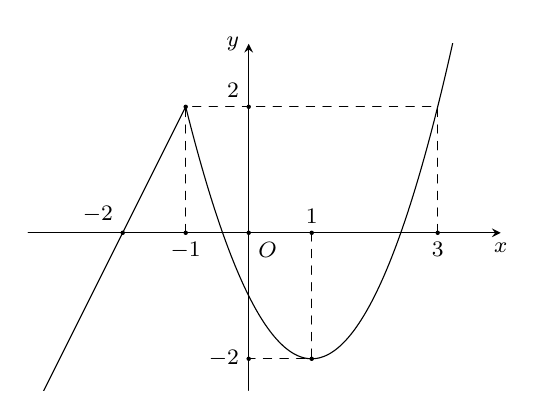
\begin{tikzpicture}[scale=0.8, font=\footnotesize, line join=round, line cap=round, >=stealth]
			\def\xt{-3.5}
			\def\xp{4}
			\def\yd{-2.5}
			\def\yt{3}
			\draw[->](\xt,0) -- (0,0)node[below right]{$O$} -- (\xp,0)node[below]{$x$};
			\draw[->](0,\yd)--(0,\yt)node[left]{$y$};
			\begin{scope}
				\clip (\xt,\yd) rectangle (\xp,\yt);
				\draw[smooth,samples=150] plot[domain=-1:\xp](\x,{(\x-1)^2-2});
				\draw plot[domain=\xt:-1](\x,{2*(\x)+4});
			\end{scope}
			\foreach \i in {(-2,0), (-1,0), (0,0), (1,0), (3,0), (0,2), (0,-2), (-1,2), (1,-2)} \fill \i circle(1pt);
			\draw[dashed](1,0)node[above]{$1$} |- (0,-2)node[left]{$-2$}
			(-1,0)node[below]{$-1$} |- (0,2)node[above left]{$2$}
			(3,0)node[below]{$3$} |- (0,2)
			(-2,0)node[above left]{$-2$};
		\end{tikzpicture}
	\end{center}
	Tính giá trị của biểu thức $T=f(-1)-2f(1)+f(3)$.
	\choice
	{$T=0$}
	{\True $T=8$}
	{$T=3$}
	{$T=2$}
	\loigiai
	{Từ đồ thị ta có $f(-1)=2$, $f(1)=-2$, $f(3)=2$. Suy ra $T=f(-1)-2f(1)+f(3) = 2+4+2=8$.}
\end{ex}

\begin{ex}%[0D3N1-5]
	\immini{Cho hàm số $y=f(x)$ có tập xác định $D=[-3;3]$ và có đồ thị như hình bên. Khẳng định nào sau đây là đúng?
	\choice
	{\True Hàm số nghịch biến trên khoảng $(-1;1)$}
	{ Hàm số đồng biến trên khoảng $(0;1)$}
	{ Hàm số nghịch biến trên khoảng $(-3;-1)$}
	{ Hàm số nghịch biến trên khoảng $(1;3)$}}
	{\begin{tikzpicture}[scale=0.75, font=\footnotesize,line join=round, line cap=round,>=stealth]
		%\def\xmin{-4} \def\xmax{4}
		%\def\ymin{-2} \def\ymax{4}
		%\draw[color=gray!50,dashed] (\xmin,\ymin) grid (\xmax,\ymax);
		\draw[->] (-3.5,0)--(0,0)node[above left]{$O$}--(3.5,0) node[below right]{$x$};
		\draw[->] (0,-1.5)--(0,4.5) node [above right]{$y$};
		\draw (-3,-1)--(-1,1)--(1,0)--(3,4);
		\draw[dashed](-3,0)--(-3,-1)--(0,-1)(-1,0)--(-1,1)--(0,1)(3,0)--(3,4)--(0,4);
		%\fill[black] (0,3.5) circle(3pt) (3,8) circle(3pt) (7,0) circle(3pt);
		%\draw (0,3.5) node[left]{\footnotesize $3.5$} (7,0) node[below]{\footnotesize $7$} (3,0) node[below]{\footnotesize $3$};
		%\shade[top color=black!80] (1,6) circle(12pt);
		%\fill[black] (0,0) circle (1pt);
		\foreach \x in {-3,...,-1,1,2,3}
		\draw (\x,0) node[below]{$ \x $};
		\foreach \y in {-1,-1,1,2,3,4}
		\draw (0,\y) node[right]{$ \y $};
		\foreach \x/\y in {3/0,2/0,1/0,0/0,-1/0,-2/0,-3/0,0/-1,0/1,0/2,0/3,0/4,3/4,-1/1,-3/-1}{\draw[fill=black] (\x,\y) circle (1pt);}
	\end{tikzpicture}}

	\loigiai{
		Dựa vào đồ thị ta thấy hàm số nghịch biến trên khoảng $(-1;1)$.
	}
\end{ex}

\begin{ex}%[Đề thi HK1 trường Song Ngữ Á Châu năm học 2023-2024]%[Trần Quang Trường, dự án 10-11EX]%[0D3N2-1]
	Trục đối xứng của đồ thị hàm số $y=ax^2+bx+c$, $(a\ne 0)$ là đường thẳng nào dưới đây?
	\choice
	{\True $x=-\dfrac{b}{2a}$}
	{$x=-\dfrac{c}{2a}$}
	{$x=-\dfrac{\Delta}{4a}$}
	{$x=\dfrac{b}{2a}$}
	\loigiai{

	}
\end{ex}

\begin{ex}%[0D3N2-3]
	\immini{Cho parabol $y=a{x^2}+bx+c$ có đồ thị như hình vẽ. Trục đối xứng của parabol trên là đường thẳng có phương trình
	\choice
	{$y=-1$}
	{$y=1$}
	{$x=0$}
	{\True $x=1$}}{	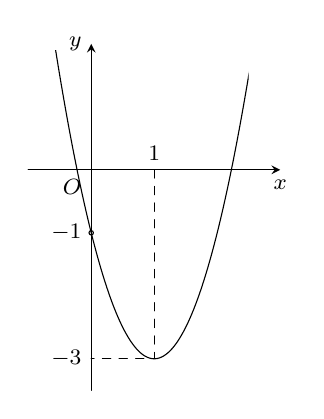
\begin{tikzpicture}[scale=0.8,>=stealth, font=\footnotesize, line join=round, line cap=round]
	\def\a{2} \def\b{-4} \def\c{-1} % Hệ số
	\def\xmin{-1} \def\xmax{3}
	\def\ymin{-3.5} \def\ymax{2}
	
	%	\draw[color=gray!50,dashed] (\xmin,\ymin) grid (\xmax,\ymax);
	
	\draw[->] (\xmin,0)--(\xmax,0) node [below]{$x$};
	\draw[->] (0,\ymin)--(0,\ymax) node [left]{$y$};
	\node at (0,0) [below left]{$O$};
	\clip (\xmin+0.1,\ymin+0.1) rectangle (\xmax-0.5,\ymax-0.1);
	\draw[smooth,samples=300] plot(\x,{\a*(\x)^2+\b*(\x)+\c});
	\draw[dashed](1,0)node[above]{$1$}|-(0,-3)node[left]{$-3$};
	\draw(0,-1)node[left]{$-1$}circle(1pt);
	\end{tikzpicture}}
	\loigiai{
	Dựa vào đồ thị ta có trục đối xứng của đồ thị là đường thẳng $x=1$.}
	\end{ex}
\Closesolutionfile{ans}

\TNTF
\Opensolutionfile{ans}[ans/ansDe2-TN2]
\begin{ex}%[0H9H3-2]
	Cho hai điểm $A(3;-3)$, $B(-1;-5)$ và đường thẳng $(d)\colon 4x-3y-2=0$.
	\choiceTF
	{\True Một vectơ chỉ phương của đường thẳng $d$ là $\overrightarrow{u}=(3;4)$}
	{Phương trình đường thẳng $AB$ là $y=3x-12$}
	{Khoảng cách từ $A$ tới $(d)$ nhỏ hơn khoảng cách từ $B$ tới $(d)$}
	{\True Cosin của góc tạo bởi $(d)$ và đường thẳng $AB$ bằng $\dfrac{2}{\sqrt{5}}$}
	\loigiai{
		\begin{itemchoice}
			\itemch  \textbf{Đúng}.\\  Vectơ pháp tuyến của  đường thẳng $d$ là $\overrightarrow{n_d}=(4;-3)$ suy ra vectơ chỉ phương  $\overrightarrow{u_d}=(3;4)$.
			\itemch \textbf{Sai}.\\ 
			Phương trình đường thẳng $AB$ có dạng $y=mx+n$ nên ta có hệ phương trình
			\[\heva{&3m+n=-3\\&-m+n=-5}\Rightarrow \heva{&m=\dfrac{1}{2}\\&n=-\dfrac{9}{2}}.\]
			Vậy phương trình đường thẳng $AB$ là $y=\dfrac{1}{2}x-\dfrac{9}{2}$.
			\itemch \textbf{Sai}.\\ Khoảng cách từ $A$ đến đường thẳng $(d)$ là  $\mathrm{d}\left(A,d\right)=\dfrac{\big|4\cdot 3-3\cdot(-3)-2\big|}{\sqrt{4^2+(-3)^2}}=\dfrac{19}{5}$.\\
			Khoảng cách từ $B$ đến đường thẳng $(d)$ là $\mathrm{d}\left(B,d\right)=\dfrac{\big|4\cdot(-1)-3\cdot(-5)-2\big|}{\sqrt{4^2+(-3)^2}}=\dfrac{9}{5}$.\\
			Vậy $\mathrm{d}\left(A,d\right)>\mathrm{d}\left(B,d\right)$.
			\itemch \textbf{Đúng}.\\  Đường thẳng $AB$ nhận $\vv{AB}=\left(-4;-2\right)$ làm một vectơ chỉ phương.\\
			Đường thẳng $(d)$ có  vectơ chỉ phương là $\vv{u_d}=\left(3;4\right)$.\\
			Vậy $\cos\left(d,AB\right)=\dfrac{\big|-4\cdot 3+(-2)\cdot4\big|}{\sqrt{\left(-4\right)^2+\left(-2\right)^2}\cdot\sqrt{3^2+4^2}}=\dfrac{2\sqrt{5}}{5}$.
		\end{itemchoice}
	}

\end{ex}

\begin{ex}%[0-HK1-CT-2-LeQuyDon-TPHCM-2324]%[VN-MT-6, Nguyễn Hữu Chung Kiên]%[0D3H1-2]
	Cho hàm số bậc nhất $f(x)$ có đồ thị đi qua điểm $A(1;0)$ và cắt trục tung tại điểm $B(0;2)$. Và hàm số bậc hai $g(x)=-x^2+2$.
	\choiceTF
	{\True Hàm số có công thức là $f(x)=-2x+2$}
	{\True Hàm số $|f(x)|$ đồng biến trên $(2;+\infty)$}
	{\True Đồ thị hàm số $g(x)$ nhận trục $Oy$ làm trục đối xứng}
	{Gọi $M$, $N$ là giao điểm hai đồ thị hàm số $f(x)$ và $g(x)$. Độ dài đoạn thằng $MN$ bằng $2\sqrt{3}$}
	\loigiai{
		\begin{itemchoice}
			\itemch \textbf{Đúng.} \\
			Vì hàm số bậc nhất nên công thức của hàm số có dạng $f(x)=ax+b$.\\
			Từ $A(1;0)$ ta có $0=a+b$ và từ $B(0;2)$ ta có $2=b$.\\
			Suy ra $a=-2$ và $b=2$.\\
			Vậy hàm số có công thức là $f(x)=-2x+2$.
			\itemch \textbf{Đúng.} \\
			Vì $|f(x)| = |-2x+2| = \heva{&-2x+2, \text{ nếu } x\leq 1\\&2x-2, \text{ nếu } x>1}$ nên $|f(x)|$ đồng biến trên $(2;+\infty)$.
			\itemch \textbf{Đúng.} \\
			Vì $g(x)=-x^2+2$ nên đồ thị hàm số $g(x)$ là một parabol bề lõm hướng xuống và có đỉnh $I(0;2)$.\\
			Do đó đồ thị hàm số $g(x)$ nhận trục $Oy$ làm trục đối xứng.
			\itemch \textbf{Sai.} \\
			Phương trình hoành độ giao điểm hai đồ thị hàm số $f(x)$ và $g(x)$ là $$-2x+2=-x^2+2 \Leftrightarrow x^2-2x=0 \Leftrightarrow x(x-2)=0 \Leftrightarrow x=0 \text{ hoặc } x=2.$$
			Vì $f(0)=2$ và $f(2)=-2$ nên $M(0;2)$ và $N(2;-2)$.\\
			Do đó $MN=\sqrt{(2-0)^2+(-2-2)^2}=2\sqrt{5}$.
		\end{itemchoice}
	}
\end{ex}
\Closesolutionfile{ans}

\TNSA
\Opensolutionfile{ans}[ans/ansDe2-TN3]
\begin{ex}%[0H9H4-3]%[Dự án đề kiểm tra Toán 11 GHKII, HKII NH23-24- Huỳnh Xuân Tín]%[Sở GH-ĐT Bắc Giang]
	Trong mặt phẳng tọa độ $O x y$, cho đường tròn $(C)\colon x^2+y^2+2 x-6 y+5=0$. Tiếp tuyến của đường tròn $(C)$ tại điểm $M(0 ; 1)$ là đường thẳng có phương trình $a x+b y+2=0$. Tính giá trị của biểu thức $T=\dfrac{b}{a}$.
	\shortans{$2$}
	\loigiai{
		Đường tròn $(C)\colon x^2+y^2+2 x-6 y+5=0$ có tâm $I(-1;3)$.\\
		Tiếp tuyến của đường tròn $(C)$ tại điểm $M(0 ; 1)$ nhận vectơ $\vec{IM}=(1;-2)$ làm vectơ pháp tuyến nên có phương trình là
		\[1(x-0)-2(y-1)+5=0\Leftrightarrow x-2y+2=0.\]
		Khi đó $a=1$, $b=-2$. Do đó $\dfrac{b}{a}=-2$.}
\end{ex}

\begin{ex}%[0H9V3-2]
	Trong mặt phẳng với hệ trục tọa độ $Oxy$, cho đường thẳng $d\colon y=ax+b$ đi qua điểm $K(1 ; 3)$ và $d$ tạo với hai tia $Ox$, $Oy$ một tam giác có diện tích bằng $6$. Tính giá trị của biểu thức $b-a$.
	\shortans{$9$}
	\loigiai{Đường thẳng $d\colon y=ax+b$ cắt tia $Oy$ tại $B(0; b)$ và tia $Ox$ tại $A\left(-\dfrac{b}{a}; 0\right)$ (với $b>0$, $a<0$).\\
		Khi đó diện tích tam giác $OAB$ là $S_{OAB}=\dfrac{1}{2}OA\cdot OB=\dfrac{-b^2}{2a}$.\\
		Từ giả thiết ta có hệ phương trình $\heva{&\dfrac{-b^2}{2a}=6\\&a+b=3.}$\\
		Giải hệ phương trình ta được $\heva{&a=-3\\&b=6}$ nên $b-a=9$.
	}
\end{ex}

\begin{ex}%[0H9V3-8]
	Theo Google Maps, sân bay Nội Bài có vĩ độ là $21{,}2^\circ$ Bắc, kinh độ $105{,}8^\circ$ Đông, sân bay Đà Nẵng có vĩ độ là $16{,}1^\circ$ Bắc, Kinh độ $108{,}2^\circ$ Đông. Một máy bay, bay từ Nội Bài đến sân bay Đà Nẵng. Tại thời điểm $t$ phút, Tính từ lúc xuất phát, máy bay ở vị trí có vĩ độ $x^\circ$ Bắc, kinh độ $y^\circ$ Đông được tính theo công thức
	\[\heva{& x=21{,}2-\dfrac{51}{800}t\\& y=105{,}8+\dfrac{3}{100}t.}\]
	Hỏi chuyến bay từ Hà Nội đến Đà Nẵng mất bao nhiêu phút?
	\shortans[]{80}
	\loigiai{
	Tại sân bay Nội Bài, máy bay bắt đầu bay ứng với thời gian $t=0$.\\
	Tọa độ của sân bay Đà Nẵng thỏa mãn hệ $\heva{&x=21{,}2-\dfrac{51}{800}t\\&y=105{,}8+\dfrac{3}{100}t.}$\\
	Do đó, thời gian máy bay bay từ Hà Nội đến Đà Nẵng là Nghiệm $t$ của hệ phương trình
	\[\heva{&16{,}1=21{,}2-\dfrac{51}{800}t\\&108{,}2=105{,}8+\dfrac{3}{100}t} \Leftrightarrow t=80.\]
	Vậy chuyến bay từ Hà Nội đến Đà Nẵng mất $80$ phút.
	}
\end{ex}

\begin{ex}%[0H9V5-0]
	\immini
	{
		Một tòa tháp (hình bên) có mặt cắt là một đường hypebol và có chiều cao $200$ m, chỗ nhỏ nhất ở chính giữa và rộng $50$ m, đỉnh tháp và đáy tháp có độ rộng đều bằng $60$ m. Độ rộng của tòa tháp ở độ cao $150$ m bằng bao nhiêu (kết quả tính theo đơn vị mét và làm tròn đến hàng phần chục)?
	}
	{
		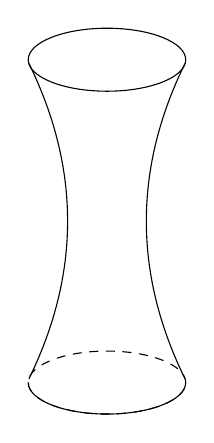
\begin{tikzpicture}[line join = round, line cap = round,>=stealth,scale=1,font=\footnotesize]
			%		\draw[->] (-2,0) -- (2,0) node[right] {$x$};
			%		\draw[->] (0,-3) -- (0,3.2) node[above] {$y$};
			\draw[domain=-2:2,smooth, samples=150] plot ({(0.35*(\x))^(2)+0.5},\x);
			\draw[domain=-2:2,smooth, samples=150] plot (-{(0.35*(\x))^(2)-0.5},\x);
			\draw (0,2.05) ellipse (1 and 0.4);
			\draw[dashed] (0,-2.05) ellipse (1 and 0.4);
			\draw (0,-2.05)+(0:1 and 0.4) arc (0:-180:1 and 0.4);
		\end{tikzpicture}
	}
	\shortans{$52{,}7$}
	\loigiai{
	\immini
	{
		Gắn hệ trục tọa độ $Oxy$ như hình bên, $1$ đơn vị đo tương ứng $1$ m.\\
		Phương trình chính tắc của hypebol $(H)\colon \dfrac{x^2}{a^2}-\dfrac{y^2}{b^2}=1,\ (a > 0, b> 0)$.\\
		Theo giả thiết ta có $2a=50\Rightarrow a=25$.\\
		Mặt khác $(H)$ đi qua $M(30;100)$ nên ta có $\dfrac{30^2}{25^2}-\dfrac{100^2}{b^2}=1\Rightarrow b^2=\dfrac{250000}{11}\Rightarrow (H)\colon \dfrac{x^2}{625}-\dfrac{y^2}{\dfrac{250000}{11}}=1$.
	}
	{
		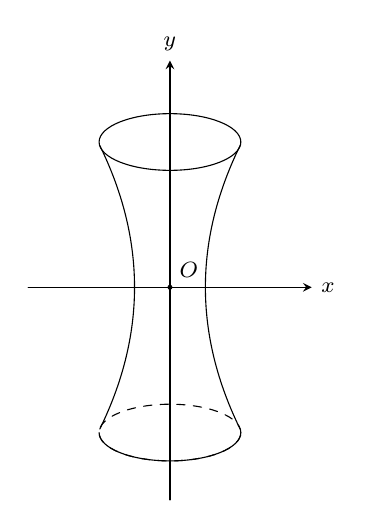
\begin{tikzpicture}[line join = round, line cap = round,>=stealth,scale=0.9,font=\footnotesize]
			\draw[->] (-2,0) -- (2,0) node[right] {$x$};
			\draw[->] (0,-3) -- (0,3.2) node[above] {$y$};
			\draw[domain=-2:2,smooth, samples=150] plot ({(0.35*(\x))^(2)+0.5},\x);
			\draw[domain=-2:2,smooth, samples=150] plot (-{(0.35*(\x))^(2)-0.5},\x);
			\draw (0,2.05) ellipse (1 and 0.4);
			\draw[dashed] (0,-2.05) ellipse (1 and 0.4);
			\draw (0,-2.05)+(0:1 and 0.4) arc (0:-180:1 and 0.4);
			\fill (0,0)node[above right]{$O$} circle (1pt);
		\end{tikzpicture}
	}
	\noindent Độ rộng của tháp ở độ cao $150$ m ứng với điểm $N(x;50)\in (H)$ nên ta có
	$$\dfrac{x^2}{625}-\dfrac{50^2}{\tfrac{250000}{11}}=1\Rightarrow x=\dfrac{5\sqrt{111}}{2}.$$
	Suy ra độ rộng của tháp ở độ cao $150$ m là $2x=\dfrac{2\cdot 5\sqrt{111}}{2}=52{,}7\ \mathrm{(m)}$.
	}
\end{ex}
\Closesolutionfile{ans}

\TL
\begin{ex}%[HKI THPT VO THI SAU]%[Vanle Vo-10-11EX-HK1-23-24]%[0D3H2-3].
	Cho hàm số $y=-x^2+4x-3$ có đồ thị $(P)$. Vẽ đồ thị $(P)$.
	\loigiai{
		\begin{itemize}
			\item Tọa độ đỉnh $S\left(2;1\right)$.
			\item Trục đối xứng $x=2$.
			\item Bảng giá trị
			      \begin{center}
				      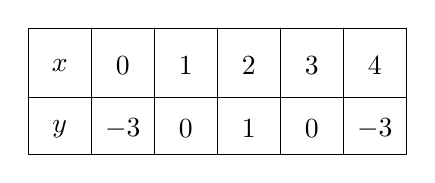
\begin{tikzpicture}[scale=0.8, line join=round, line cap=round,>=stealth]
					      \def\a{6} % số nhãn chiều dài
					      \def\b{2} % số nhãn chiều cao
					      \draw[shift={(-.5,.5)},black]
					      (0,0.1) rectangle +(\a,-\b)
					      (0,-1)--+(0:\a) ;
					      \foreach \x/ \tren in {0/$x$,1/$0$,2/$1$,3/$2$,4/$3$,5/$4$}
					      \draw (\x,0) node{\tren};
					      \foreach \y/ \duoi in {0/$y$,1/$-3$,2/$0$,3/$1$,4/$0$,5/$-3$}
					      \draw (\y,-1) node{\duoi};
					      \foreach \z in {.5,1.5,2.5,3.5,4.5,5.5}
					      \draw (\z,0.6)--(\z,-1.4) ;
				      \end{tikzpicture}
			      \end{center}
			\item Đồ thị
			      \begin{center}
				      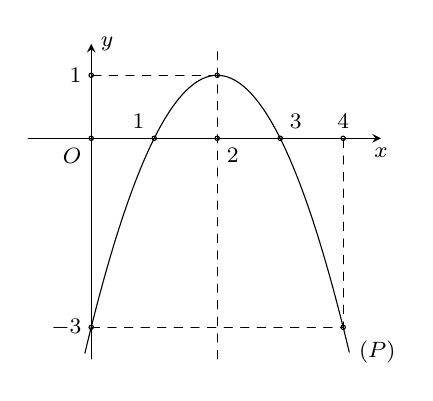
\begin{tikzpicture}[line join=round,line cap=round, font=\footnotesize,scale=0.8,>=stealth]
					      \draw[-stealth] (-1,0)--(4.6,0) node[below] {$x$};
					      \draw[-stealth] (0,-3.5)--(0,1.5) node[right] {$y$};
					      \draw (0,0)circle(1pt) node [below left] {$O$};
					      %%Vẽ các điểm trên 2 hệ trục
					      \draw (1,0)circle(1pt) node [above left] {$1$}
					      (4,0)circle(1pt) node[above] {$4$}
					      (2,0)circle(1pt) node [below right] {$2$}
					      (3,0)circle(1pt) node [above right] {$3$}
					      (0,-3)circle(1pt) node[left] {$-3$}
					      (0,1)circle(1pt) node[left] {$1$}
					      (4,-3)circle(1pt)(2,1)circle(1pt);
					      %%Vẽ đỉnh và trục đối xứng
					      \draw[dashed, thin] (0,-3)--(4,-3)--(4,0) (2,-3.5)--(2,1.5)(2,1)--(0,1);
					      \draw[samples=350,smooth,variable=\x] plot[domain=-0.1:4.1] (\x,{-1*(\x)^2+4*(\x)-3})node [right] {$(P)$};
				      \end{tikzpicture}
			      \end{center}
		\end{itemize}
	}
\end{ex}

\begin{ex}%[0H9V3-8]
	Một sân bay cần xây dựng một đường băng thẳng nối hai điểm $A(3; 1)$ và $B(9; 7)$ trên bản đồ quy hoạch đã được gắn hệ trục tọa độ. Một tháp kiểm soát không lưu được xây dựng tại vị trí $C(6; 2)$. Hãy kiểm tra xem khoảng cách này có lớn hơn $5$ km không (để đảm bảo quy định an toàn)?
	\loigiai{
		Phương trình đường thẳng $AB$ nhận $\overrightarrow{AB}=(6;6)$ làm vectơ chỉ phương nên đường thẳng $AB$ có một vectơ pháp tuyến là $\overrightarrow{n}=(1;-1)$.\\
		Khi đó, đường thẳng $AB$ có phương trình là $1\cdot (x-3)-1\cdot (y-1)=0\Leftrightarrow x-y-2=0$.\\
		Khoảng cách từ điểm $C(6;2)$ đến đường thẳng $AB$ là
		\[\mathrm{d}(C,AB)=\dfrac{\left|6-2-2\right|}{\sqrt{1^2+(-1)^2}}=\sqrt{2}<5.\]
		Vì khoảng cách nhỏ hơn $5$ km, tháp kiểm soát không lưu không đảm bảo quy định an toàn.
	}
\end{ex}

\begin{ex}%[Nguyễn Cường- BG Toán 10]%[0D2T2-5]
	Nồng độ cồn trong máu $(BAC)$ được định nghĩa là phần trăm rượu (rượu ethyl hoặc ethanol) trong máu của một người. $BAC$ là $ 0{,}05 \%$ có nghĩa là có $0{,}05$ gam rượu trong $100 \mathrm{ml}$ máu. Càng uống nhiều rượu bia thì nồng độ cồn trong máu càng cao và càng nguy hiểm khi tham gia giao thông. Nồng độ $BAC$ trong máu của một người được thể hiện qua đồ thị sau:
	\begin{center}
		\begin{tikzpicture}[>=stealth, line join=round, line cap=round, font=\footnotesize, scale=1,yscale=.75]
			\draw[->] (-1,0)--(0,0)node[below left]{$O$}--(7,0)node[below]{$t$ (giờ)};
			\draw[->] (0,-1)--(0,5)node[left]{$BAC$ ($\%$)};
			\draw[dashed](3,0)node[below]{$1$}--(3,2)--(0,2)node[left]{$0{,}068$};
			\draw (0,3)node[left]{$0{,}076$}--(6,1);
			\fill[black](3,2)circle (1pt);
		\end{tikzpicture}
	\end{center}
	\begin{listEX}[1]
		\item	Viết công thức biểu thị mối quan hệ giữa nồng độ cồn trong máu $(BAC)$ sau $t$ giờ sử dụng.
		\item Theo nghị định 100/2019/ND-CP về xử phạt vi phạm hành chính, các mức phạt (đối với xe máy). Hỏi sau $3$ giờ, nếu người này tham gia giao thông thì sẽ bị xử phạt ở mức độ nào?
	\end{listEX}
	\begin{center}
		\begin{tabular}{|l|c|}
			\hline
			Mức $1$: Nồng độ cồn chưa vượt quá $50$mg/$100$ml máu        & Phạt tiền từ $02-03$ triệu đồng \\&(tước bằng từ $10-12$ tháng) \\
			\hline
			Mức $2$: Nồng độ cồn  vượt quá $50$mg đến $80$mg/$100$ml máu & Phạt tiền từ $04-05$ triệu đồng \\&(tước bằng từ $16-18$ tháng)\\
			\hline
			Mức $3$: Nồng độ cồn vượt quá $80$mg/$100$ml máu             & Phạt tiền từ $06-08$ triệu đồng \\&(tước bằng từ $22-24$ tháng) \\
			\hline
		\end{tabular}
	\end{center}
	\loigiai{
		\begin{enumerate}
			\item Dựa vào đồ thị ta gọi công thức biểu thị mối liên hệ giữa nồng độ cồn trong máu $(BAC)$ sau $t$ giờ sử dụng có công thức $BAC=at+b$.\\
			      Từ đồ thị ta có hàm số đi qua các điểm $(0;0{,}076)$ và $(1;0{,}068)$ nên ta được
			      $\heva{& BAC=0{,}076 \\ & a=-\dfrac{1}{125}.}$\\
			      Công thức biểu thị mối quan hệ giữa nồng độ cồn trong máu $(BAC)$ sau $t$ giờ sử dụng là $BAC=-\dfrac{1}{125}t+0{,}076$.
			\item Nồng độ cồn trong máu sau $3$ giờ là $BAC=-\dfrac{1}{125}\cdot 3+0{,}076=0{,}052$.\\
			      Do nồng độ cồn trong máu sau $3$ giờ là $0{,}052$mg/$100$ml máu nằm ở mức $2$ nên người này bị phạt tiền từ $04-05$ triệu đồng  và tước bằng từ $16-18$ tháng.
		\end{enumerate}
	}
\end{ex}

% \HetDe
% \label{De2}
% %
% \cleardoublepage
% \setcounter{page}{1}
% \rfoot{Trang \thepage/\pageref{DA2} - Đáp án trắc nghiệm Mã đề 2}
% \begin{center}
% 	\bfseries ĐÁP ÁN TRẮC NGHIỆM MÃ ĐỀ 2
% \end{center}

% \inputansbox{10}{ans/ansDe2-TN1}
% \inputansbox[3]{2}{ans/ansDe2-TN2}
% \inputansbox{3}{ans/ansDe2-TN3}
% \label{DA2}
%
